\documentclass[a4paper,UTF8]{article}
\usepackage{amsmath}
\usepackage{amssymb}
\usepackage{amsthm}
\usepackage{bm}
\usepackage{color}
\usepackage{ctex}
\usepackage{enumerate}
\usepackage[margin=1.25in]{geometry}
\usepackage{graphicx}
\usepackage{hyperref}
\usepackage{tcolorbox}
\usepackage{algorithm}
\usepackage{algorithmic}
\theoremstyle{definition}
\newtheorem*{solution}{Solution}
\newtheorem*{prove}{Proof}
\newcommand{\indep}{\rotatebox[origin=c]{90}{$\models$}}
\usepackage{multirow}              

\setlength{\evensidemargin}{.25in}
\setlength{\textwidth}{6in}
\setlength{\topmargin}{-0.5in}
\setlength{\topmargin}{-0.5in}
% \setlength{\textheight}{9.5in}
%%%%%%%%%%%%%%%%%%此处用于设置页眉页脚%%%%%%%%%%%%%%%%%%
\usepackage{fancyhdr}                                
\usepackage{lastpage}                                           
\usepackage{layout}                                             
\footskip = 12pt 
\pagestyle{fancy}                    % 设置页眉                 
\lhead{2020年春季}                    
\chead{机器学习导论}                                                
% \rhead{第\thepage/\pageref{LastPage}页} 
\rhead{作业四}                                                                                               
\cfoot{\thepage}                                                
\renewcommand{\headrulewidth}{1pt}  			%页眉线宽,设为0可以去页眉线
\setlength{\skip\footins}{0.5cm}    			%脚注与正文的距离           
\renewcommand{\footrulewidth}{0pt}  			%页脚线宽,设为0可以去页脚线

\makeatletter 									%设置双线页眉                                        
\def\headrule{{\if@fancyplain\let\headrulewidth\plainheadrulewidth\fi%
		\hrule\@height 1.0pt \@width\headwidth\vskip1pt	%上面线为1pt粗  
		\hrule\@height 0.5pt\@width\headwidth  			%下面0.5pt粗            
		\vskip-2\headrulewidth\vskip-1pt}      			%两条线的距离1pt        
	\vspace{6mm}}     								%双线与下面正文之间的垂直间距              
\makeatother  


\begin{document}
\title{机器学习导论\\
	习题四}
\author{191300020, 黄彦骁, AdrianHuang@smail.nju.edu.cn}
\maketitle


\section*{学术诚信}

本课程非常重视学术诚信规范,助教老师和助教同学将不遗余力地维护作业中的学术诚信规范的建立。希望所有选课学生能够对此予以重视。\footnote{参考尹一通老师\href{http://tcs.nju.edu.cn/wiki/}{高级算法课程}中对学术诚信的说明。}

\begin{tcolorbox}
	\begin{enumerate}
		\item[(1)] 允许同学之间的相互讨论,但是{\color{red}\textbf{署你名字的工作必须由你完成}},不允许直接照搬任何已有的材料,必须独立完成作业的书写过程;
		\item[(2)] 在完成作业过程中,对他人工作(出版物、互联网资料)中文本的直接照搬(包括原文的直接复制粘贴及语句的简单修改等)都将视为剽窃,剽窃者成绩将被取消。{\color{red}\textbf{对于完成作业中有关键作用的公开资料,应予以明显引用}};
		\item[(3)] 如果发现作业之间高度相似将被判定为互相抄袭行为,{\color{red}\textbf{抄袭和被抄袭双方的成绩都将被取消}}。因此请主动防止自己的作业被他人抄袭。
	\end{enumerate}
\end{tcolorbox}

\section*{作业提交注意事项}
\begin{tcolorbox}
	\begin{enumerate}
		\item[(1)] 请在\LaTeX模板中{\color{red}\textbf{第一页填写个人的姓名、学号、邮箱信息}};
		\item[(2)] 本次作业需提交该pdf文件、问题1,2可直接运行的源码(nn.py, DF21.py,{\color{red}\textbf{不需要提交数据集}}),将以上三个文件压缩成zip文件后上传。zip文件格式为{\color{red}\textbf{学号.zip}},例如190000001.zip;pdf文件格式为{\color{red}\textbf{学号\_姓名.pdf}},例如190000001\_张三.pdf,{\color{red}\textbf{并通过教学立方提交}}。
		\item[(3)] 未按照要求提交作业,或提交作业格式不正确,将会{\color{red}\textbf{被扣除部分作业分数}};
		\item[(4)] 本次作业提交截止时间为{\color{red}\textbf{5月25日23:55:00。}}
	\end{enumerate}
\end{tcolorbox}

\newpage


\section{[55pts] Neural Networks in Practice}

\par 在训练神经网络之前,我们需要确定的是整个网络的结构,在确定结构后便可以输入数据进行端到端的学习过程。考虑西瓜书第101-102页以及书中图5.7中描述的神经网络,即:输入是$ d $维向量$ \mathbf{x}\in\mathbb{R}^d $,隐藏层由$ q $个隐层单元组成,输出层为$ l $个输出单元,其中隐层第$ h $个神经元的阈值用$ \gamma_h $表示,输出层第$ j $个神经元的阈值用$ \theta_j $表示,输入层第$ i $个神经元与隐层第$ h $个神经元之间的连接权重为$ v_{ih} $,隐层第$ h $个神经元与输出层第$ j $个神经元之间的连接权重为$ w_{hj} $,记隐层第$ h $个神经元接收到的输入为$ \alpha_h=\sum_{i=1}^{d}v_{ih}x_i $,输出为$ b_h=f(\alpha_h-\gamma_h) $,输出层第$ j $个神经元接收到的输入为$ \beta_j=\sum_{h=1}^{q}w_{hj}b_h $,输出为$ \hat{y}_j=f(\beta_j-\theta_j) $,$ f $为对应的激活函数。

\begin{enumerate}[(1)]
	\item \textbf{[30 pts(编程题)]} 若隐层单元和输出层单元的激活函数都是$Sigmoid$函数,使用均方误差作为网络的损失函数(见西瓜书式(5.4))。请打开\textbf{nn.py}程序并完成以下任务:完成Sigmoid 函数及其梯度函数的编写,完成MSE损失函数和accuracy函数的编写,完成NeuralNetwork() 类中向前传播predict函数,以及train函数的编写,其中包括向前传播、梯度计算、更新参数三个部分。对测试集完成尽量准确的分类预测(accuracy到0.5以上即可)。每轮梯度下降时,使用所有样本做累积BP算法,更新梯度时使用样本的平均梯度。请截图汇报测试集的MSE和Accuracy。

	      请注意,你需要基于numpy实现模型,除了示例代码中使用到的sklearn库函数,你将不允许使用其他sklearn函数。为方便并行计算,请使用numpy的矩阵/点积/均值/求和等函数而不是for循环进行运算,如果结果正确但使用了for循环,将会酌情扣分。
	\item \textbf{[20 pts]} 神经网络学习分类问题时,模型输出层更加常用的设置是$ Softmax $加交叉熵损失,即:假定隐层单元的激活函数是$Sigmoid$函数不变,对输出层,令$ z_j=\beta_j-\theta_j $,则输出为$ \hat{y}_j=\frac{e^{z_j}}{\sum_{i=1}^{l}e^{z_i}} $,损失函数$ E=-\sum_{j=1}^{l}y_j\log{\hat{y}_j} $,$ y_j $为该输出对应真实标记。请给出此时的梯度$ \frac{\partial{E}}{\partial{w_{hj}}} $,$ \frac{\partial{E}}{\partial{\theta_{j}}} $,$ \frac{\partial{E}}{\partial{v_{ih}}} $和$ \frac{\partial{E}}{\partial{\gamma_{h}}} $。(需给出计算步骤,可以像西瓜书一样定义新的符号$ g_j$、$e_h $,但已有符号需使用题目中给定符号表示)
	\item \textbf{[5 pts]} 相比依次直接求$ v,\gamma $和$ w,\theta $的梯度,简述BP算法在计算上的优点?

\end{enumerate}

\begin{solution}
	\begin{enumerate}
		\item [(1)]mse和acc:
		      \begin{figure}[h]
			      \centering
			      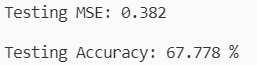
\includegraphics[width=7cm,height=2cm]{mse_and_acc.png}
			      \caption{mse和acc}
		      \end{figure}
		\item [(2)]首先对梯度进行化简:
		      \[\frac{\partial{E}}{\partial{w_{hj}}} = (\sum_{i=1}^{l}\frac{\partial{E}}{\partial{\hat{y_i}}}\frac{\partial{\hat{y_i}}}{\partial{\beta_j}})\frac{\partial{\beta_j}}{\partial{w_{hj}}}\]
		      \[\frac{\partial{E}}{\partial{\theta_j}} = -\sum_{i=1}^{l}\frac{\partial{E}}{\partial{\hat{y_i}}}\frac{\partial{\hat{y_i}}}{\partial{\beta_j}}\]
		      \[\frac{\partial{E}}{\partial{v_{ih}}} = \frac{\partial{E}}{\partial{b_h}}\frac{\partial{b_h}}{\partial{\alpha_h}}\frac{\partial{\alpha_h}}{\partial{v_{ih}}}\]
		      \[\frac{\partial{E}}{\partial{\gamma_h}} = - \frac{\partial{E}}{\partial{b_h}}\frac{\partial{b_h}}{\partial{\alpha_h}}\]
		      令:
		      \[g_j = \sum_{i=1}^{l}\frac{\partial{E}}{\partial{\hat{y_i}}}\frac{\partial{\hat{y_i}}}{\partial{\beta_j}} = \sum_{i\neq j}^{l}y_i\hat{y}_j - (1-\hat{y}_j)y_j = \hat{y}_j\sum_{i=1}^{l}y_i - y_j\]
		      \[e_h = \frac{\partial{E}}{\partial{b_h}}\frac{\partial{b_h}}{\partial{\alpha_h}} = b_h(1-b_h)\sum_{j=1}^{l}\frac{\partial{E}}{\partial{\beta_j}}\frac{\partial{\beta_j}}{\partial{b_h}} = b_h(1-b_h)\sum_{j=1}^{l}w_{hj}g_j\]
		      故有:
		      \[\frac{\partial{E}}{\partial{w_{hj}}} = g_jb_h\]
		      \[\frac{\partial{E}}{\partial{\theta_j}} = -g_j\]
		      \[\frac{\partial{E}}{\partial{v_{ih}}} = e_hx_i\]
		      \[\frac{\partial{E}}{\partial{\gamma_h}} = -e_h\]
		\item[(3)]BP算法在计算上更加快捷简便,同时保留中间梯度变量,对后续其他计算也能提供帮助,同时编程时更加便捷
	\end{enumerate}
\end{solution}


\section{[10pts(编程题)] Deep Forest in Practice}

\par 深度森林是周志华老师等提出的新型深度学习模型。2021年2月1日,深度森林软件包DF21开源发布\footnote{\url{https://deep-forest.readthedocs.io/en/latest/}},它拥有比其他基于决策树的集成学习方法更好的性能,更少的超参数,并且无需大量的调参,训练效率高。请安装DF21,并参考\textbf{DF21.py},在波士顿房价预测数据上比较DF21 和sklearn 随机森林的性能,汇报两个模型在测试集上的Mean Square Error (MSE),以及将DF21 的n\_estimators 超参数在不同取值(大于等于3个取值)时的测试集MSE绘制成折线图。(由于模型和数据划分有随机性,可以直接用跑一次的结果,也可取跑多次的均值)

\begin{solution}
	比较深度森林与随机森林的mse:
	\begin{figure}[h]
		\centering
		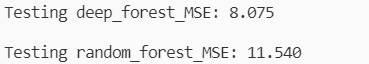
\includegraphics[width=7cm,height=2cm]{mse_deep_random.png}
		\caption{mse对比}
	\end{figure}
	可以看出深度森林的mse要显著小于随机森林,后续多次实验得到结果也印证了这一点.

	mse曲线:见图二
	\begin{figure}[t]
		\centering
		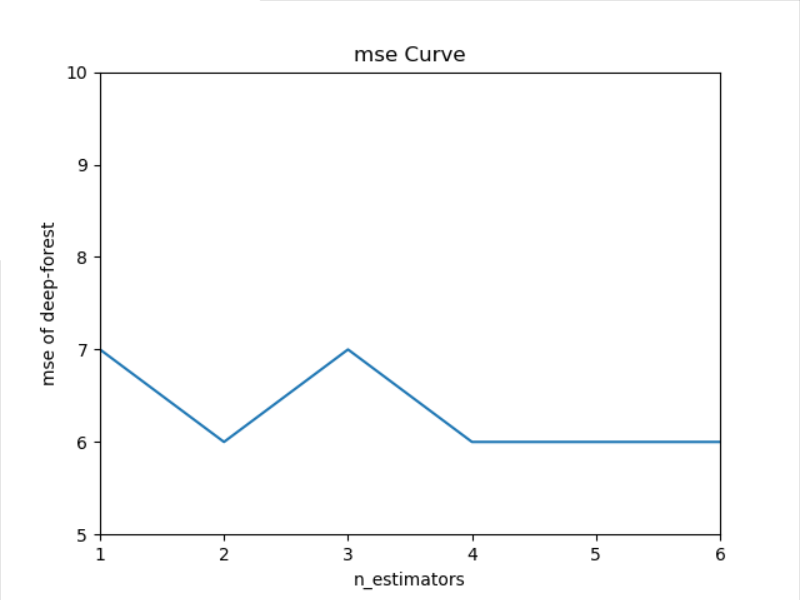
\includegraphics[width=8cm,height=6cm]{mse_curve.png}
		\caption{mse曲线}
	\end{figure}
\end{solution}

\section{[35 pts] Naive Bayes Classifier}

\par 通过对课本的学习,我们了解了采用“属性条件独立性假设”的朴素贝叶斯分类器。现在我们有如下表所示的一个数据集,其中$x_1$与$x_2$为特征,其取值集合分别为$x_1=\{-1,0,1\}$,$x_2=\{B,M,S\}$,y为类别标记,其取值集合为$y=\{0,1\}$:
\begin{table}[htp]
	\centering
	\caption{数据集}\label{tab:aStrangeTable}
	\begin{tabular}{cccccccccccccccc}
		\hline
		编号  & $1$ & $2$ & $3$ & $4$ & $5$ & $6$ & $7$ & $8$ & $9$ & $10$ & $11$ & $12$ & $13$ & $14$ & $15$ \\
		\hline
		$x_1$ & -1  & -1  & -1  & -1  & -1  & 0   & 0   & 0   & 0   & 0    & 0    & 1    & 1    & 1    & 1    \\
		\hline
		$x_2$ & $B$ & $M$ & $M$ & $B$ & $B$ & $B$ & $M$ & $M$ & $S$ & $S$  & $S$  & $M$  & $M$  & $S$  & $S$  \\
		\hline
		$y$   & 0   & 0   & 1   & 1   & 0   & 0   & 0   & 1   & 1   & 1    & 1    & 1    & 1    & 1    & 0    \\
		\hline
	\end{tabular}
\end{table}

\begin{enumerate}[(1)]
	\item \textbf{[5pts]}通过查表直接给出的$x=\{0,B\}$的类别;
	\item \textbf{[15pts]} 使用所给训练数据,学习一个朴素贝叶斯分类器,并用学习得到的分类器确定$x=\{0,B\}$的标记,要求写出详细计算过程;
	\item \textbf{[15pts]} 使用“拉普拉斯修正”,再学习一个朴素贝叶斯分类器,以及重新计算$x=\{0,B\}$的标记,要求写出详细计算过程。
\end{enumerate}


\begin{solution}
	\begin{enumerate}
		\item [(1)] 直接找到表内编号为6的样本满足$x=\{0,B\}$,所以其类别为0.
		\item [(2)] 首先根据表中数据估计先验概率:
		      \[P(y=0)=\frac{2}{5},P(y=1) = \frac{3}{5}\]
		      然后计算每个属性对应属性值的条件概率:
		      \[P(x_1=-1|y=0) = \frac{1}{2},P(x_1=0|y=0)=\frac{1}{3},P(x_1=1|y=0)=\frac{1}{6}\]
		      \[P(x_1=-1|y=1)=\frac{2}{9},P(x_1=0|y=1)=\frac{1}{3},P(x_1=1|y=1)=\frac{4}{9}\]
		      \[P(x_2=B|y=0)=\frac{1}{2},P(x_2=M|y=0)=\frac{1}{3},P(x_2=S|y=0)=\frac{1}{6}\]
		      \[P(x_2=B|y=1)=\frac{1}{9},P(x_2=M|y=1)=\frac{4}{9},P(x_2=S|y=1)=\frac{4}{9}\]
		      由上述条件进行预测:
		      \[P\left(y=0 \mid x_{1}=0, x_{2}=B\right)=P(y=0) P\left(x_{1}=0 \mid y=0\right) P\left(x_{2}=B \mid y=0\right)=\frac{1}{15}\]
		      \[P\left(y=1 \mid x_{1}=0, x_{2}=B\right)=P(y=1) P\left(x_{1}=0 \mid y=1\right) P\left(x_{2}=B \mid y=1\right)=\frac{1}{45}\]
		      由于$\frac{1}{15}>\frac{1}{45}$,所以朴素贝叶斯分类器将样本$x=\{0,B\}$预测为$y=0$类.
		\item [(3)]加入拉普拉斯修正后,公式变为:
		      \[\hat{P}(c)=\frac{\left|D_{c}\right|+1}{|D|+N}\]
		      \[\hat{P}\left(x_{i} \mid \mathrm{c}\right)=\frac{\left|D_{c,x_{i}}\right|+1}{\left|D_{c}\right|+N_{i}}\]
		      故先验概率变为:
		      \[\hat{P}(\mathrm{y}=0)=\frac{7}{17}, \hat{P}(\mathrm{y}=1)=\frac{10}{17} \]
		      修正后各属性值的条件概率为:
		      \[\hat{P}\left(x_{1}=-1 \mid y=0\right)=\frac{4}{9} \quad \hat{P}\left(x_{1}=0 \mid y=0\right)=\frac{1}{3} \quad \hat{P}\left(x_{1}=1 \mid y=0\right)=\frac{2}{9}\]
		      \[\hat{P}\left(x_{1}=-1 \mid y=1\right)=\frac{1}{4}, \hat{P}\left(x_{1}=0 \mid y=1\right)=\frac{1}{3}, \hat{P}\left(x_{1}=1 \mid y=1\right)=\frac{5}{12}\]
		      \[\hat{P}\left(x_{2}=B \mid y=0\right)=\frac{4}{9}, \hat{P}\left(x_{2}=M \mid y=0\right)=\frac{1}{3}, \hat{P}\left(x_{2}=S \mid y=0\right)=\frac{2}{9}\]
		      \[\hat{P}\left(x_{2}=B \mid y=1\right)=\frac{1}{6}, \hat{P}\left(x_{2}=M \mid y=1\right)=\frac{5}{12}, \hat{P}\left(x_{2}=S \mid y=1\right)=\frac{5}{12}\]
		      由此继续预测得:
		      \[\hat{P}\left(y=0 \mid x_{1}=0, x_{2}=B\right)=\hat{P}(y=0) \hat{P}\left(x_{1}=0 \mid y=0\right) \hat{P}\left(x_{2}=B \mid y=0\right)=\frac{28}{459} \]
		      \[\hat{P}\left(y=1 \mid x_{1}=0, x_{2}=B\right)=\hat{P}(y=1) \hat{P}\left(x_{1}=0 \mid y=1\right) \hat{P}\left(x_{2}=B \mid y=1\right)=\frac{5}{153}\]
		      由于$\frac{28}{459}>\frac{5}{153}$,故样本被预测为$y=0$类。
	\end{enumerate}
\end{solution}



\end{document}